
\chapter{Motivation}
\label{chp:motivation}

Computer aided tools for plastic surgery serve as the external
motivation for the work presented in this document. In this chapter,
this idea will be explored more thoroughly. The goals of this chapter
are twofold: first, we will formalize and review the concept of
plastic surgery simulation by studying the various aspects and
requirements of such systems. As we will see, there exist many
subtleties of both plastic surgery training itself, and the task of
simulating it on a computer. Second, this chapter will attempt to
bring these ideas into a general conceptual framework, showing how
they can be used in more areas beyond surgical simulation and how
these systems can drive research. Combined, these two discussions will
motivate the importance and utility of the technical contributions
presented in later chapters.

\section{Medical Simulation: Requirement Specification}

When exploring computer science research with a domain specific focus,
such as we are doing here with plastic surgery simulation, it is
critical to understand the expectations of domain experts. Not only do
these expectations guide the development of software, but they can
help triage research goals and serve as domain appropriate metrics for
the evaluation of final results. In this section, we will explore the
specific requirements of our domain, specifically craniofacial plastic
surgery, while keeping practical engineering considerations in
mind. In the process, we will begin developing a framework in
which these requirements can be placed and will be explored further in
later sections.

To accomplish this goal, we need answer a series of questions that
define the scope of our proposed tools, as well as its metrics for
success: What is the potential real-world utility of the tool? How
well does the system accomplish the task it was designed for?  What
are the fine grained aspects of the required tasks? What features need
to implemented (or perhaps more interestingly, not implemented)? Who
are its users? We will answer these questions by looking more narrowly
at the problem of medical simulation for craniofacial operations which
we have chosen for our benchmark.

For the purposes of this document, the range of craniofacial
operations under consideration will be restricted to ``local flap''
procedures~\citep{Baker:2014}. These procedures locally alter the
geometry of skin tissue, but do not include any alterations to
underlying bones or muscle layers. Nor do they involve any remote
effects, such as tissue grafts. These procedures are fundamental
building blocks of more complex operations, but, due to their often
non-intuitive geometry, can be difficult to learn. In fact, these
procedures often have natural analogs in computer graphics and
geometry.

\begin{figure}
  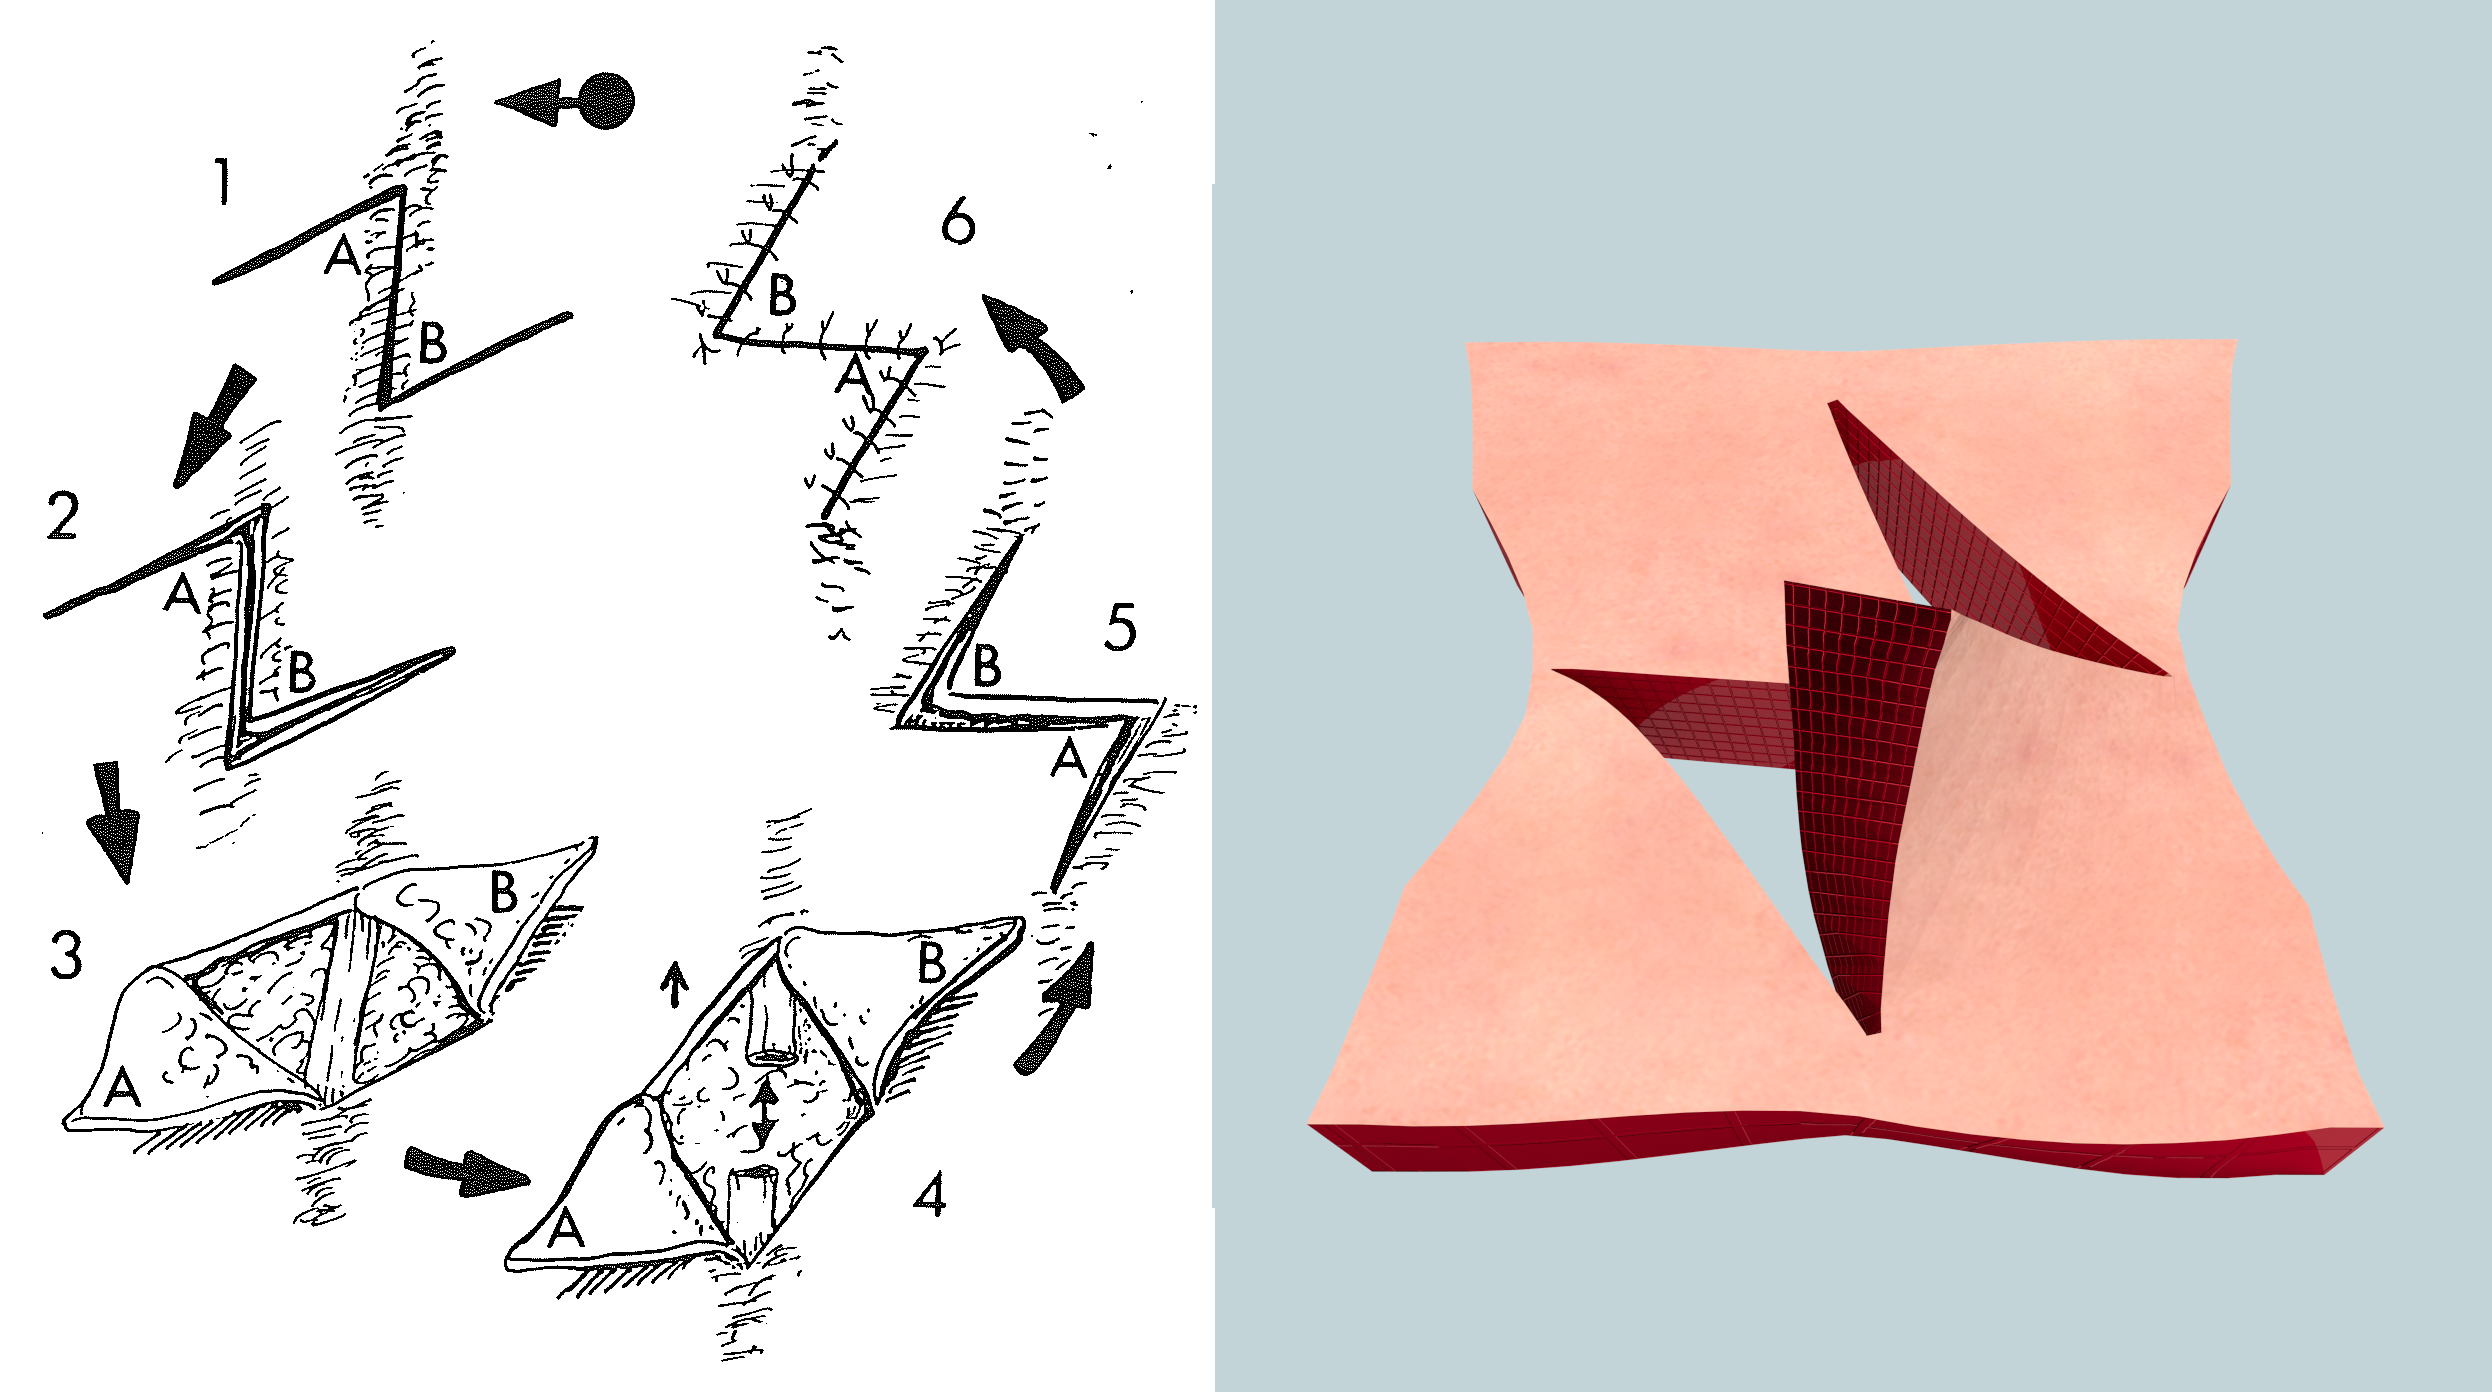
\includegraphics[width=\textwidth]{chapter_gridiron/images/zPlastyComparison.png}
  \vspace*{-.05in}
  \caption{Z-plasty: Comparison between textbook illustration and simulation}{A
    comparison between the classic \textit{Z-plasty} operation from a standard
    textbook ~\citep{McCarthy1990} (left) and a simulated version of the procedure
    in three dimensions (right). The simulation allows for
    more of the three dimensional shape of the procedure to be
    appreciated.}
  \vspace*{-.05in}
  \label{fig:ZPlastyComparison}
\end{figure}

Graphics practitioners would associate these elementary actions with
geometric transforms: shear, rotation, uniform or anisotropic
scaling. Of course, applying such transformation on live tissue is
very different than their application on a geometric model. When
stretching a tissue patch in one direction to $125\%$ of its original
length while contracting it in the transverse direction down to
$80\%$, squeezing-and-stretching in-place is typically \emph{not} the
desired way to execute this transform. Real skin might not stretch
that far or buckle in the transverse direction during the process. A
maneuver called the \emph{Z-plasty} (see Figure
\ref{fig:ZPlastyComparison}, right) achieves the same net effect, with
a more graceful stress distribution and a smooth blend to the
surrounding tissues. In plastic surgery, \textit{cognitive training}
addresses the mental challenge of how these elemental surgical
puzzle-pieces are individually designed and how they can be assembled
into larger, more complex operations. Unfortunately, 3D computer-based
cognitive training solutions for facial reconstructive surgery are
virtually nonexistent; common educational materials are limited to 2D
sketches (see Figure \ref{fig:ZPlastyComparison}, left) and still
photographs of procedures.

Surgical skills targeted by computer-based training solutions have
been classified \cite{GallaRCHFMSS:2005} in two major
categories. Psychomotor skills refer to the dexterous use of the
surgeon's hands to manipulate instruments in the course of an
operation. In plastic surgery, psychomotor training involves
mechanical aspects of surgical tasks, such as the ``feel'' of tissue
being cut or the nuances of manipulating a scalpel to enact a curved
incision. For example, training for laparoscopic procedures requires a
clinician to be familiar with the tactile response of pushing and
pulling on organs and to practice coordination skills required for
suturing and cauterization.  A number of computer-based solutions
focus on psychomotor training, including the works of
\cite{MendoL:2003,DeKLS:2005,KimCDS:2007,LindbT:2007}.  In contrast to
psychomotor training, \emph{cognitive} skills and training are largely
mental rather than dexterous exercises. For example, in the procedure
shown in Figure \ref{fig:gridiron-teaser}, the surgeon needs to
contemplate how to best repair a large square skin defect (i.e. area
of excised tissue) by making auxiliary incisions that create properly
shaped ``puzzle pieces'' which can be sutured together without
creating excessive stress. As an example of a cognitive training
system,~\cite{ChentARCHGSO:2009} described a cognitive training system
for steerable needle insertion, where the mental challenge lies in
planning a sequence of actions involving needle flexion and torsion,
in order to achieve a desired insertion trajectory.

\begin{figure}
  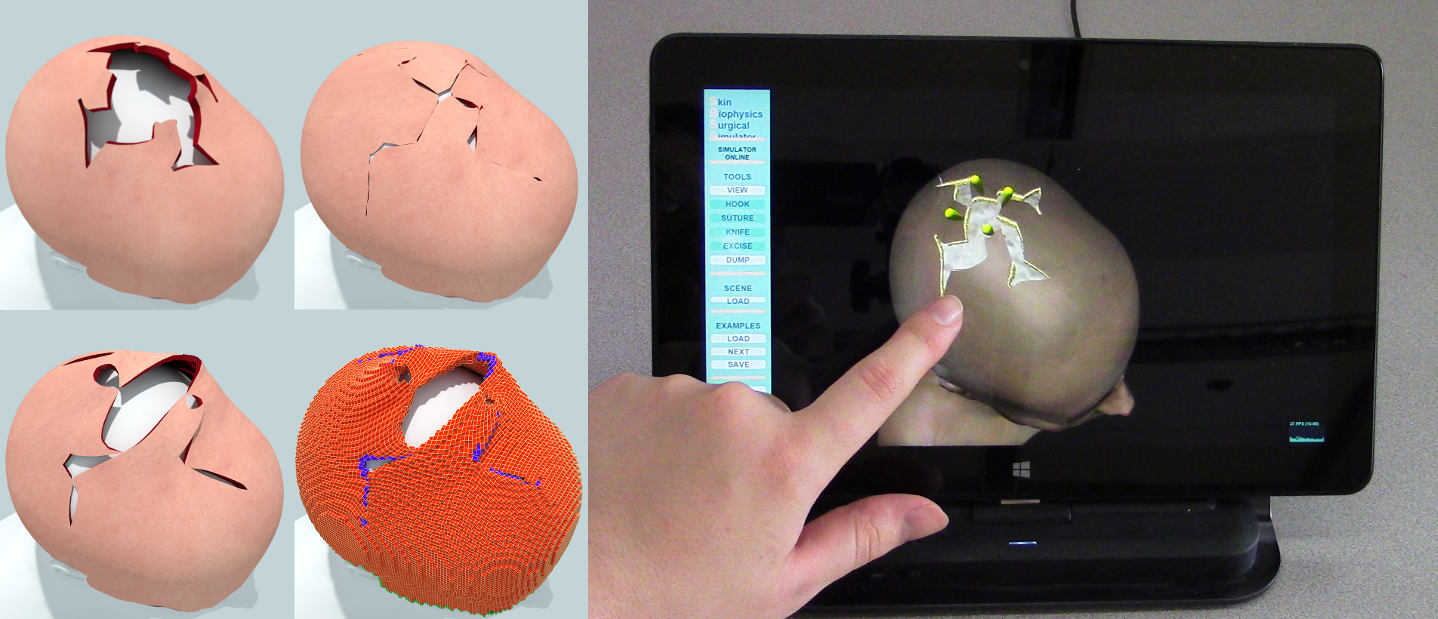
\includegraphics[height=2.99in]{chapter_gridiron/images/TitleImage.png}
  \vspace*{-.05in}
  \caption{Simulation of an advanced surgical repair at the top of the
    scalp}{Simulated \textit{Dufourmentel-Mouly} repair (see\
    \protect\cite{Baker:2014}) for a large gap of excised tissue on
    the scalp. From top to bottom, left to right: Rendered stages of
    procedure, embedding lattice, real time demo on a tablet running
    in a web browser.}
  \vspace*{-.05in}
  \label{fig:gridiron-teaser}
\end{figure}

Focusing on any individual type or aspect of skill training affects
the design decisions of a proposed tool. For instance, building a
system for psychomotor training likely places a greater emphasis on
the interactivity aspects of the system, potentially requiring haptic
feedback mechanisms to provide tactile sensations. Likewise, a
cognitive training aid might require more involved reactivity and
dynamism, such as a more accurate representation of tissue
behaviors. Ultimately, our goal should be to construct a virtual aid
which resembles reality as much as possible, in order to support all
training goals. In our pursuit of this gold standard, we need to take
the opportunities as they arrive to target particular aspects of
surgical training. In this case, we find ourselves in a position to
handle important cognitive training tasks, even if we have to
compromise on psychomotor skills.

This document will present techniques for supporting a cognitive
simulation for plastic surgery. In particular, the goal is to support
an authoring tool which supports the following basic tasks: design
local flap operations on interactive, virtual tissue models, record
and playback operations for the purpose of knowledge retention and
review, and support limited training potential. It is not the
immediate goal of this work to present a training tool in which user's
actions are graded, nor do we claim a predictive model, where all
tissue responses are accurate enough to use as a basis for real
surgery decisions. Instead, the tool should simply allow an
experienced practitioner to capture their knowledge of procedures in
an interactive, visual environment and to pass that knowledge onto
others.

In order to further refine the ultimate shape of this proposed
simulation aid, we will now look at five important aspects as they
relate to plastic surgery simulation: Geometry, Reactivity, Dynamics,
Interactivity, and Utility. In the following section, we will see how
these ideas can be generalized.

\paragraph{Geometry} Surgery in general, plastic surgery in
particular, are areas in medicine which depend strongly on a
practitioner's intuitive spatial reasoning processes. At a high level,
the task of a plastic surgeon is to manipulate the geometry of the
human body into a new configuration. The reasons for this style of
intervention are numerous and range from cosmetic procedures,
post-operation repairs, and fixing congenital deformities. Contrary to
popular public perception, plastic surgery is often employed to enact
functional repairs. Those living with injuries and deformities often
have difficulties because the specific geometry of their condition
adversely affects the proper functioning of their body. A surgeon must
understand the geometry of their patient in order to produce both
functionally correct, but also aesthetically pleasing, outcomes. Since
these operations are often highly visible, failures or mistakes can be
extremely costly in an emotional and social sense for the patient, let
alone a continued disability. Any tool designed for this domain must
take these concerns seriously and present a compelling visual
representation.

The work presented in this document achieves this goal by describing a
tool for visually authoring plastic surgery operations in a three
dimensional virtual environment. However, it is worth taking time to consider
some potential alternatives. For instance, a two dimensional sketching
interface could be considered, drawing on the rich history of surgical
instructional diagrams that exist in the field. Certainly such
approaches have been used for decades in surgical textbooks, but they
fall short of giving the viewer a comprehensive perspective of the
inherent three dimensional nature of human anatomy. Alternatively, one
might consider using video of real operations, annotated with
information describing what is happening. While this idea certainly
leaves no question about the three dimensionality of the problem, it
does so by sacrificing the clarity a rendered computer model can
provide and the ability to alter the geometry easily.

A note should also be made on display technology. Here the word
``display'' should be treated loosely and should be taken to mean any
physical channel which conveys information from the tool to the
user. Commonly, this is restricted to visual interfaces, such as
computer monitors or \glspl{hmd}. However, it could also refer to
force feedback devices, where a user receives tactile responses from
their actions in the system. Ultimately, the proper device choice for
a surgical simulation aid depends on its intended purpose. Many commercial
tools for training surgeons on laparoscopic equipment use a tightly
coupled visual and tactile feedback system. The goal of these tools is to
replicate operating room conditions exactly, hopefully instilling into
physicians the \gls{tacit} required.

\paragraph{Reactivity and User Interaction}

The display of three dimensional, static tissue geometry is an
improvement over the two dimensional illustrations commonly employed
in training literature. However, in order to provide surgeons more
realism, we also need to have the models react to their inputs. In
real surgeries, there exist many ways a surgeon might interact with
human tissue: injecting drugs, cutting it, applying suction to remove
blood, and suturing it together are all candidate interactions. For
the purposes of this document, and to focus on the cognitive aspects
of manipulating tissue geometry, we will be focusing on three types of
user interactions: pulling on tissue, joining tissue together, and
changing its topology. These concepts map directly to surgical tasks,
namely using surgical hooks to pull tissue around, adding sutures to
close wounds, and cutting into tissue with a scalpel. This subset of
interactions, while small, is still capable of expressing many
interesting operations, particularly in regard to the cognitive
problem solving scenarios we wish to target. The ability for users to
cut, pull, and join enables them to explore arranging the complex
tissue geometries required for local flap procedures. We then use
physical simulation to compute a mechanical response to these user
inputs, which can be visualized by deforming the geometry of the
tissue model.

By creating a cause and effect relationship between the user's input
and the tissue's shape through simulation, we can provide users an
environment in which to learn more about how their proposed procedures
might perform in reality. By leaving the simulation flexible, we can
also allow for later integration of realistic biomaterial
behaviors. These materials are extremely complex and often behave in
non-intuitive, time dependent fashions. While their accurate simulation
is beyond the scope of this document, we want to not exclude the
possibility of including them later.

\paragraph{Dynamics}

It is worth discussing at this point the nature of \textit{time} with respect
to our proposed tool, which can often be non-intuitive. The real-world
phenomena we are representing are heavily dependent on time in two
major ways: sequencing and lag-based effects. Sequencing refers to the
nature of cause and effect, specifically the relative ordering of
events and the time taken between them. In the real world, we can
generally think of the allowed user actions ( i.e. cutting, pulling,
joining) as being naturally ordered and smoothly continuous in
time. For our purposes, we will relax this concept in our benchmark
tool to allow for discrete events. While we maintain that user actions
should remain ordered, as we wish to track the steps of an operation,
we will record these actions as a series of discrete states. This is
not fundamentally different than the idea of discrete stages of an
illustrated operation, as we saw in Figure \ref{fig:ZPlastyComparison}
earlier. As we transition between input states, the simulation will
gradually converge to a new mechanical response, creating the illusion
of dynamic motion.

However, we need to be careful to distinguish between this illusion of
motion and real dynamic lag effects. These effects are commonly
expressed in real materials as jiggling, but can also be seen in
surgical contexts in the form of swelling or other physiological
reactions to tissue damage. We will be specifically avoiding these
types of dynamic behavior in our tool for several reasons. First, the
models describing these behaviors are extremely complex and
delicate. Moreover, the right answer to these problems are not clear
yet in all cases. Second, even if we had a well defined model,
computing dynamic effects is computationally expensive, which could
harm the interactivity of our tool. Finally, we don't really need
perfect resolution of these effects to initially accomplish our goal of
cognitive training, which involves more careful planning rather than
immediate reactions to dynamic effects. 




% This last point brings up the question of time and how the concept of
% time interacts with user input. Time is a critical factor
% during real surgery - beyond the life threatening aspects of taking
% too long, tissue also undergoes physiological reactions such as
% swelling and fluid loss, which alter its mechanical
% behaviors. Tracking these states is beyond the scope of this work. In
% fact, we are proposing a mostly time invariant environment - where the
% shape of the tissue only depends on the current state of the user's
% input\footnote{This is a slight simplification. User actions which
%   change the topology of the tissue should be considered ordered in time. It
%   is physically implausible to simply replace tissue that has been previously
% cut away.}. To avoid simply snapping from one state of mechanical
% response to another, we additionally propose that the simulation
% should gradually blend between states. More about how this can be
% accomplished will be discussed in Chapter \ref{chp:engineering} and
% elsewhere in this document.


% \paragraph{Reactivity \& Dynamism} During their education, a surgeon
% builds intuitions relating to the various tissues of the human
% body. Primarily, they are interested in how the tissues, such as skin,
% react to external forces: pulling and pushing. These biomaterials
% behave in complex and often non-intuitive fashions, which must be
% internalized into a surgeon's mental model of an operation. When
% considering a virtual representation of an operation, maintaining
% these properties for a user in the face of their real-life experience
% is important. Incorporating these behaviors into a system typically
% falls under the ideas of reactivity and dynamism.

% This document will show how these properties can be generated by
% simulating elastic materials, but this is not the only approach that
% could be taken. To avoid the computational expense of physics
% simulation, one might consider traditional animation. Here, a trained
% animator might work closely with a surgical domain expert to develop
% three dimensional animations. These animations would move in the
% correct fashion, stretching and bulging where appropriate. However,
% they would behave in a fixed fashion, perhaps embodying a series of
% finite states. The primary benefits of this approach are flexibility
% and speed. The creative team behind the animations can do what they
% want, unrestricted by anything except their imagination and knowledge
% of real-world behaviors. Additionally, once created, the animations
% can be played back at high speed requiring, compared to simulation,
% few computational resources. Unfortunately, this requires sacrificing
% the ability to make dynamic changes and requires significant time
% commitment from the artists and surgeons.

% While traditional animation techniques can capture the reactive
% qualities of human tissue, physical simulation better captures the
% dynamic aspects, especially when reactivity and dynamism are mixed. An
% example to consider are the effects of blood loss on tissue. Undamaged
% human tissue is composed primarily of water, a material which is
% largely imcompressible. Accordingly, human tissue can also be thought
% of as effectively incompressible - until a surgeon cuts into it. As
% blood leaves through the open wound, the water content of surrounding
% tissue drops resulting in the tissue becoming more and more
% compressible. This a \textit{dynamic} property of the
% tissue. Depending on how quickly a surgeon works, the subsequent
% manipulations may be on tissue that is more or less compressible
% changing the way they \textit{react}. Physical simulation excels at
% capturing this complex interplay between reactive behavior dynamic
% properties, which can only be roughly approximated by prescribed animations.

% Unfortunately, incorporating all dynamic aspects of human tissue into
% a simulation is impractical. For this stage, we instead choose to
% focus on the elastic properties of the tissue, foregoing effects such
% as swelling. While these effects can significantly affect the course
% of an surgical operation, the primary focus of this work is the
% geometry of the procedures. By addressing the challenges of providing
% a user manipulable tissue surface, the work in this document can
% provide a solid foundation for future improvements which bring more
% natural tissue dynamics into the simulation.  


% \paragraph{Interactivity} Surgeons require impressive hand-eye
% coordination; they carefully trained over many years on how to
% interact with human tissue, both manually and via surgical
% instruments. A substantial challenge in developing a virtual surgical
% aid is how to map these complex modes of interaction to a computer
% system while retaining usefulness. There are many approaches than can
% be taken to reconcile this challenge, depending on the ultimate goals
% of the application. If the goal is to provide the user with realistic
% physical sensations, haptic feedback interfaces can be used. Many
% existing surgical simulation tools in the industry and in academic
% circles have used this
% technique~\citep{KimCDS:2007,DeKLS:2005,MendoL:2003,LindbT:2007}.
% Alternatively, it might be more important to replicate the exact
% environment a surgeon might encounter. Often this utility is desired
% in cases where the surgeon is learning unfamiliar equipment or needs
% training in exotic interfaces, such as laparoscopic
% systems~\citep{SUSAC:2002--2014}.

\paragraph{Utility} 

The final topic to discuss is the planned utility of the tool,
specifically the expected use cases and deployment concerns. As
mentioned previously, our goal to support users in authoring scenarios for
local flap operations. The planned modes of interaction are
two-fold. First is the authoring mode, where an experienced user will
interact with a three dimensional, simulated tissue model to sequentially
plan a procedure. This will be accomplished by using the mouse and
keyboard to select tools (i.e. cutting, pulling, and joining) and apply
them to the surface of the model. As each tool is applied and recorded, the
simulation will update providing the user with the results of their
last input. The second mode is the playback, or viewing, mode. In this
mode, the user, potentially a student, will select a pre-authored
procedure from an available database. At this point, the user will be
allowed to advance through the procedure one step at a time, where the
steps are the prerecorded inputs from the previous authoring
mode. During both modes of operation, the user will have freedom to move the
model around in virtual space, allowing them to see all aspects of the
manipulation at every stage.

In addition to the two modes of operation, we want the tool to support
a multi-user shared environment. This will allow the tool to support
scenarios such as classroom settings or shared presentations. Under
this concept, multiple users will be able to connect clients to a
remote simulation server and observe the same scene. Each client will
be permitted their own independent view point, allowing the same
freedom to look at the deforming model as before. However, the
simulation will be shared and the effects of any input entered by any
user will be propagated to every other connected client. The remote
simulation server should be designed to run as one of the clients or
as a wholly separate device, allowing it to be customized for
additional performance or upgraded later. In comparison, the user
clients should be lightweight, allowing for easy deployment across a
wide range of available platforms.




% The final aspect to discuss in regards
% to the plastic surgery domain is that of utility. This topic has been
% touched upon in the previous sections on Geometry, Reactivity,
% Dynamism, and Interactivity. However, the goal here is to explore how
% such a system can be used to support the plastic surgery
% profession. In the beginning of this section, we discussed the
% difference between cognitive and psychomotor skills, as well as the
% concept of an authoring tool. However, the need for such a tool hasn't
% been clearly defined yet.

% It should be clear how an authoring tool can support surgical
% education: By supporting interactive, three dimensional illustrations,
% such a tool can augment and replace the classical training literature
% describing procedures. A simulation tool as wide applicability,
% whether the use case is a private tool for personal review, or as a
% medium for an instructor to demonstrate a procedure to a wide
% audience. However, the utility of the idea extends beyond these
% classical training modes.

% One emerging area where a visual authoring tool could be beneficial is
% in telemedicine. This application has remote doctors or surgeons,
% often specialists, provide assistance to local practitioners through a
% variety of technological mediators. Recent studies of telemedicine for
% plastic surgery ~\citep{VyasHSMTPVMGDG2017} have shown positive
% results. However, the approaches trialed thus far have relied on
% diagnosises based on photographic evidence and either verbal or
% form-based recommendations. Allowing remote surgeons to author
% recommended approaches virtually could vastly improve knowledge
% transmission between physically separated sites.   

% Another major utility of the authoring tool is knowledge
% retention. While many techniques have been recorded in literature,
% experienced surgeons can carry decades of first hand knowledge in
% their minds. While having them train the next generation of
% practitioners can help diffuse this knowledge into the general
% community, giving them a virtual surgical sketchpad with which to
% record their ``geometric'' notes could also be a valuable method of
% preserving knowledge. 


\section{Simulation Assisted Visual Systems}

While assisting the plastic surgery community, by improving their
available methods for teaching and preparing for surgery, through
computer simulation is certainly valuable, additional value can be
gained by understanding how the previous section's concepts generalize
to a larger class of applications. This generalized class can be
referred to broadly as Simulation Assisted Visual Systems
(SAVS). These systems are characterized by their \textit{use of both physical
simulation and interactive visuals to support practical tasks}. Such
visual systems are commonplace in our modern society, though we do
not often think of them in these terms. Concrete examples include
video games, animation tools, and virtual avatar systems, though many
more could be named. The goal of this section is to define the basic
concepts underpinning these systems, particularly in respect to physics
based simulation. This deconstruction will be followed by a
examination of the challenges that exist when developing a such a system,
along with a short defense of their worth beyond their targeted
domains.

\subsection{SAVS Deconstruction}

The core of a SAVS is a virtual world, or environment. When discussing
a SAVS, we are talking about artificially constructed settings, often
completely described by a computer program and displayed via some
device. This is contrast to other simulated environments which are
built entirely in the real-world, such as police training courses for
example. However, a SAVS is not completely disconnected from
reality. In order to support a user in a particular task, a SAVS is
often designed to mimic real life situations. Returning to the
definition above, is it appropriate to declare any virtual environment
a SAVS? Not exactly - building on their proposed definition, we can
structure a SAVS according to a series of important properties, or
\textit{aspects}. These aspects should be familiar from the previous
section: Geometry, Reactivity, Dynamics, Interactivity, and
Utility. However, now we will demonstrate how these aspects are
expressed in a more generic sense instead of the surgical context from
earlier.

\begin{description}
\item[Geometry] The Geometry of a SAVS refers to anything within the
  system dealing with shape or visual appearance. This is an
  intentionally broad concept, including geometry representation,
  texturing, and how these topics can be used functionally within the
  system. Ultimately, the greatest challenge with the geometry aspect
  is our own desires. Like the legend of King Midas, we must be
  careful to reign in our never ending need for more detail, in the
  form of more refined meshes, higher resolution textures, or higher
  resolution discretizations, or we run the risk of negatively
  impacting the overall system. Visual detail comes with steep costs,
  whether in the form of computational time required to render images,
  the storage space hold the information, or in the time required by
  artists to manually create assets. However, improved visuals are not
  simply an optional feature. If we give them up for the sake of
  performance or simplicity, we risk being unable to appreciate the
  results of the system in a satisfying manner. Worse, we might
  adversely affect the system's simulation components by producing
  discrete models too coarse to capture the important continuous
  mechanical properties. In the end, visual detail needs to be
  balanced between our wants and what we can afford, while paying
  close attention to what we choose to comprise the result of the
  choice.

\item[Reactivity] Reactivity describes the ability of a SAVS to hold
  state and allow its users to change this state meaningfully via
  interactions with the system. In terms of simulation, reactivity
  also captures the concept of boundary conditions, material models,
  and contact behaviors. In the benchmark application described
  earlier, our boundary conditions were limited to user defined hooks
  or point-to-point joins. In general, the types of boundary
  conditions vary - from spatial spline curves~\citep{SetalWMKS:2014}
  to attaching virtual bones to simulated muscles~\citep{PatteMS:2012,MitchCS:2015}. The
  primary challenge with boundary conditions is determining how to
  best translate the intuitive control we are used to in the
  real-world into simulation friendly alternatives. It is easy to
  demand the ability to push on a squishy simulated object, but
  reconciling that specification with the specific discretizations
  employed or remaining robust throughout the process can be
  challenging. Similarly complex are the available material models for
  simulated objects. While a fairly standard set of materials were
  chosen for the surgical application, in order to facilitate
  performance and robustness, more exotic models exist that exhibit
  properties like plasticity and
  viscoelasticity~\citep{WojtaT:2008}. Additionally, contact handling
  is a large part of reactivity - the choice of including it or not,
  and whether or not collision free guarantees are required can
  dramatically affect the results of a simulation. The choice of
  including some or all of these features into a system can provide
  more control on the part of the user, but it is important to avoid
  adding so much that the performance or robustness of the system is
  negatively affected. Instead, these reactivity features should be
  selected for the utility they bring to the system.

  % This aspect critically enables many
  % other useful properties of a SAVS. First, it brings an
  % important property of determinism to the system. Instead of static
  % or random reactions, users should expect their actions will produce
  % understandable (yet not necessarily simple!) consequences. Second,
  % this property defines the rules of the SAVS, which are
  % important both to the designer and the user. The designer needs to
  % understand the rules in order to make informed choices and
  % compromises in development (more on this later). The user of the
  % system needs the rules, even implicitly stated, to gain intuitions
  % and learn how to use the system. If these rules faithfully replicate
  % real world behaviors, the user may be able to translate knowledge
  % learned from the SAVS into the physical world.
  
\item[Dynamics] As we discussed earlier, Dynamics refers to the
  effects of time in a system. For our surgical simulation benchmark,
  we have chosen to do without many dynamic behaviors to improve
  robustness and performance. However, dynamics are often an important
  property to retain in other use cases. For instance, dynamic
  jiggling of soft material can be highly desirable in character
  animation, where lifelike motion is often closely linked with this
  highly visual behavior. Advanced animation use cases might require
  non-linear or anisotropic damping models, depending on the
  underlying material composition and character design~\citep{Xu:2017:EBD}.


  %Materials like steel, which can
  %exhibit fracturing under repeated bending, might need to be
  %simulated using dynamics to capture potentially disastrous failure
  %modes for buildings or bridges.

  

\item[Interactivity] Interactivity refers to two concepts: the overall
  speed or performance of the system and the methods that a user has
  to interact with it. With regards to simulation, we can talk about
  the concept of a time-sensitive simulation. Under this regime, we
  have a limited budget of time before we must display a new visual
  frame to the user. Video games are a classic example of this idea,
  where high frame rates are desirable to provide a smooth and
  immersive experience. Simulations used in video games are under
  extremely tight constraints in terms of time per simulation
  step~\citep{ParkeO:2009}. This problem also be thought of as lag, or
  the time between when a user performs and action and when they see a
  change from the simulation. This issue only becomes exaggerated when
  introducing remote simulations, where the network becomes an
  additional lag source in the system. Video games have generally
  handled this problem by locally predicting game state into the
  future and interpolating new information as it arrives, but this
  technique is difficult for simulation based systems as good future
  predictions are on the same order of complexity as the simulation itself.

  The other side of interactivity is the user controls. For
  simulation, control is generally achieved via user manipulable
  boundary conditions, potentially creating additional reactivity
  requirements within the system. But in general, user controls exist
  to either serve a technical function, such as the abstract
  manipulators in geometric modeling environments, or to improve the
  immersiveness, such as the hand and body tracking technologies being
  explored in video games. The proper choice of input mechanisms
  depends on the intended use of the system and can greatly shape a
  user's impressions of the system.

\item[Utility] We touched on some high level examples of Utility
  earlier, citing video games and animation tools, but in general the
  reason we use simulation in a SAVS is to impart some aspect of
  mechanical realism into a virtual environment. The term mechanical
  is being used here to refer to objects which behave according to
  physical laws, not that we are restricting ourselves to only
  simulating machinery. And certainly there are many applications
  which benefit from these behaviors. Video games can use simulation
  to create procedurally destructible environments~\citep{ParkeO:2009}
  and animators use modeling tools to create lifelike character motion
  through flesh simulation~\citep{McAdaST:2010}. More complex
  simulations are regularly used to predict mechanical behaviors in
  advance of manufacturing, saving both time and money during
  development.
      
\end{description}

\subsection{SAVS Challenges}

Designing a Simulation Assisted Visual System comes with a wide
array of challenges, which is not especially surprising when
considering how many components can be included into their
framework. In this section, some of these challenges will be reviewed,
hopefully to provide better context for the design decisions that were
made for the rest the work presented in this document.

\subsubsection{No One Size Fits All?}

Reusability is commonly described in software engineering as an
important design concept, but comes with a particular set of
challenges in a SAVS. In general, the idea is that reusable components
in a software system are desirable as the work required for their
creation can be amortized among multiple client systems.  Designing a
SAVS imposes some interesting roadblocks for the principle of
reusability.

The first issue that often comes up is that the
requirements for a SAVS, while they can appear similar in structure
(e.g. display a 3D environment, respond to user input, simulate
materials, etc.), are often implemented with specific optimizations
due to the tight restrictions placed on such systems (e.g. near
real-time performance, extremely complex environments,
etc.). Developers faced with these issues can easily fall into the
trap of \textit{blind optimization}. This is a form of anti-pattern~\citep{antipatterns:1998}, where they optimize the implementation,
often quite expertly, for some aspect but without considering the rest
of the system, or later reusability. It is important to distinguish
this from \textit{premature optimization}, where the developer spends
time optimizing an implementation before knowing if such effort is
required. Blind optimization is performed under local
justification. It is only with a broader context that it can be
determined to be a wise course of action. Premature optimization may
end up being wasted effort at best, detrimental at worst. In a
simulation context, these activities can result in rigid components,
such as material models or solvers, which deliver high performance but
are not adaptable or easy to swap out for new functionality. These are
issues the work in this document has attempted to avoid. 

Even if we ignore optimization, the fundamental design choices baked
into simulation systems can make them difficult to reuse. Often, in
the pursuit of supporting a particular physical property (e.g. strong
incompressibility), choices are made in the mathematical formulation or
data structures that preclude other properties from easily
coexisting. The challenge here is in identifying these restricting
choices early, either to avoid them or to understand their effect on
potential future development activities. Ignoring the consequences can
easily lead to situations where an implementation is abandoned simply
because it will not function well with other techniques, instead of 
any inherent mistake or flaw in its own design.

Designing general purpose SAVS platforms is not impossible. Game
developers, over a long developmental history, have created many
excellent general platforms for game development, referred to as game
engines. But increasingly, these platforms, and the developers who
design them, are becoming a field in their own right.  In the past, a
game developer might have done everything from writing low level
graphics code to higher level game logic. In contrast, modern games
are often written by developers who know little about the low level
optimizations required to reach the fidelity and performance expected
by current audiences. Instead, these skills are expressed in game
engines - highly tuned, carefully optimized systems which are not a
game per se, but act as a solid foundation for games written on top of
them. They provide \textit{services}: rendering, resource management,
network support, user interface toolkits, and much more. In essence,
this divide is not dissimilar to that of applications and operating
systems.

The work completed in this document generally follows this
philosophy. As will be described in later sections, the systems
presented in this work adhere to two general principles.

\begin{enumerate}
\item \textbf{Avoid Uncalled for Optimization} During implementation
  of techniques presented in this document, care was taken to avoid
  optimizing too soon. By doing so, we avoided excessive
  specialization until the design goals could be cleared stated. In
  fact, many design goals are still unclear, so a maintainable, if not
  fully optimized, system can be an advantage.
  
\item \textbf{Enforce Clean Separation} As will be discussed in more
  detail in Chapter \ref{chp:deployment}, the domain specific
  motivation, plastic surgery, was separated as much as possible from
  the underlying enabling technologies. This allowed a coupled, but
  functionally isolated, system design, where the components needed to
  build a plastic surgery simulation were isolated from the components
  needed to build a high performance finite element simulator.
  
\end{enumerate}


\subsubsection{Realism and Cruciality}

For the simulation underlying the virtual environment of a SAVS, one
primary concern is the balance between the concepts of realism and
cruciality. Realism is a direct measure of how much a user of a system
sees what is being presented as an accurate simulacra, in terms of the
mechanical behavior, of a real object or environment. Here we are
making an assumption, which should be intuitively justifiable, that
real world mechanics are the highest standard of correctness
possible. If we were capable of simulating these behaviors with
perfect accuracy, all users should be satisfied with the results. And
yet, the nature of our simulations fundamentally requires that they
are an approximation of reality. One goal of simulation research and
building a SAVS is dealing with the issue of cruciality, the
process of identifying which features, or behaviors, of reality are
most crucial to supporting the primary, user-oriented tasks of the
system. Every application has a different set of crucial features
which help define it uniquely. For the purposes of cognitive surgical
training, we are interested in simulated behaviors including
smoothness of motion, maintaining surface details, supporting contact
scenarios, and inextensiblity of materials. Real tissue, in contrast,
supports many more behaviors such as incompressibility,
viscoelasticity, and material failure under high strain - but these
are not crucial to our task. Attempting to support them in order to
improve realism both takes away developmental resources and
unnecessarily increases complexity.


% For the visual detail and virtual world aspect of a SAVS, one primary
% question that arises is one of believability versus realism. These
% concepts are often conflated, though they really should be considered
% separately.  In contrast, believability is the measure of
% how much a user trusts, or is willing to accept, the information being
% presented. Let us use modern special effects in movies as an
% example. On one hand, special effects can be used to introduce
% elements that have direct, real world counterparts, which are either
% too expensive or impractical to use. Examples might include simulating
% a full ocean, using a green screen to replace environments, or
% employing full simulation of real people. If done well, these
% techniques increase realism, by convincing the audience that the
% elements being fabricated really exist. On the other hand, special
% effects can introduce clearly fantastical elements: mythical
% creatures, exotic environments, or magical effects. These are elements
% that even the least critical audience member would not hesitate to say
% are fake. But the goal here is not convince them that the object or
% effect is real, but to convince them that it is \textit{plausible}:
% that the fire breathing dragon, if it were to really exist, would look
% just like it does on the screen. This is the believability aspect at
% work. Of course, there is no reason that realism and believability can
% not work together. Examples include live action heroic characters
% being replaced by animated versions in order to have them perform
% impossible stunts. Here the result must have realism (it looks like
% the real person), but also be believable (the impossible stunt looks
% like it could have been pulled off by the actor).

% So what does this mean for SAVS designs in general? And for medical
% simulation specifically? The primary issue with a SAVS is that of user
% input. While a movie can be scripted and refined until realism and
% believability is exactly where the actors and artists want it to be, a
% SAVS must produce similar levels of fidelity when faced with arbitrary
% user actions. Dealing with this challenge often requires domain
% specific knowledge in order to limit the potential space of user
% interactions. For example, in a surgery simulation, the user is not
% allowed do absolutely anything to a section of simulated tissue. They
% are forced, by the context of the situation, to interact with it using
% the simulated tools provided: scalpels, sutures, etc... This allows a
% surgery SAVS to be engineered to properly handle all the potential
% outcomes of this restricted interface, to better produce realistic and
% believable results.

\subsubsection{Design Conflicts}

A major problem facing the construction of any SAVS is that of design
goal conflicts. This is a common software development problem, where
supporting one feature or aspect of a system, such as performance,
comes into direct conflict with implementing another
feature. Continuing with the performance example, suppose we wanted to
impose a strict amount of time between visual updates to the user. By
doing so, we have restricted our updates with an upper bound on the
maximum amount of work they can complete at any one interval due to
these time restrictions. This choice may bias further choices towards
the use of other techniques, not because of any technical merit, but
due to computational complexity.

Many of these conflicting goals exist, some of which are well known in
general software design circles. In the context of physical
simulation, there are several conflicts we need to be especially aware
of.


\paragraph{Lag Vs. Accuracy}
Before, we touched on the ideas of reactivity and interactivity when
discussing the nature of cause and effect within a SAVS, but related
idea is known as lag. Lag is defined here to be the time between when
a user applies some change to a simulated system (a force impulse, a
constraint change, etc...) and when the user sees the result of the
action\footnote{This should be contrasted with the concept of
  hysteresis, where the effects of a stimulus naturally lag behind the
  cause. What we are talking about with lag is an \textit{artificial}
  delay which stems from algorithmic or computational artifacts.}. The
smaller this time, the more reactive the simulation \textit{feels}. We
can see this when comparing the simulation to real materials. For real
objects, the lag is effectively zero.

Of course, real materials have an advantage that simulated materials
do not. Because they are composed of individual atoms, real objects
act as a nearly continuous finite element simulation, where the elements are
almost infinitely small and operate completely in parallel to each
other. Computer simulated materials are much coarser in their
resolution and, despite great advances in parallel processing, do not
come close to that naturally available in real materials. As we
increase a simulated object's resolution in order to capture more and
more detail, or use more complex elements that capture more
interesting macroscopic effects, the overall lag of the
simulation increases as more effort is spent resolving each user
action.

The challenge is to find the appropriate balance between the desired
lag of a simulation and the accuracy of the simulation. A major
focus of this work has been to explore how both of these aspects can be
tackled simultaneously, both by exploiting underutilized parallelism
opportunities and by looking at novel data structures to extract
additional effective resolution without significantly doing so.
  
\paragraph{Domain Utility Vs. Generality}

Another two ideas that often find themselves in conflict for
physical simulation systems are the concepts of domain utility and
generality. Lets look at domain utility first, as it's the more
straightforward of the two. In the simplest terms, domain utility
refers to design choices in a system that primary serve the
specific task, or domain, that it is currently being built for. This
may refer to choosing or discarding certain features, deciding what
API best suits the current task, or making optimization along critical
paths for the client application. All of these choices can be
reasonable, even correct, as long as you never intend to reuse the
system for any other purpose.

Generality, on the other hand, asks what is the commonality of
different tasks and guides design choices along this route. A general
design should be flexible to different and changing requirements. Such
a system typically eschews APIs built for specific tasks and instead
tries to distill out the fundamental building blocks that any
potential client may need from the system. The difficulties with this
philosophy are two-fold. First, it isn't always obvious what the
fundamental interfaces are, partially because designers by necessity
must look at past applications to define them and can only make
educated guesses about future ones. But secondly, general designs
often cannot make the simplifying assumptions allowed by having domain
specific knowledge. These designs are often left with an awkward choice
between overly complex code that tries to optimize for every use case
or simpler universal code which doesn't optimize anything.

On the surface, general systems seem harder to build effectively and
often don't result in well optimized solutions, impacting other
aspects such as interactivity. The short answer is flexibility. For a
well studied domain, where every last detail is known and accounted
for, a specialized system is probably the best choice. But in order to
answer challenging research questions, tools and problems often have
to change quickly and in unexpected directions as researchers adapt to new
findings and explore new ideas. Medical simulation is very much
one of these areas, where new questions are constantly arising and old
preconceptions are abandoned. As such, during the implementation of
the systems described in this document, considerable effort was spent
on creating generalized simulation systems, and attempting to identify
which areas are ready for optimization and which were not.

 
\subsection{A Rationale for Developing a SAVS}

Despite the complexity involved in designing and implementing SAVS
type systems, the practice of developing them has significant benefits
both inside and outside of academic practice. This can be seen when
comparing them with the traditional academic development model.
Designing isolated experiments for academic pursuits in computer
science is a time tested approach for performing research. This
methodology is designed to control for unknown factors during
experiments - certainly this is what other scientific disciplines
teach as the proper approach. However, there can be significant value
in building a large system as the primary research platform. In order to
support this claim, let us look at the three avenues by which a
SAVS creates value: As a Catalyst, By Filling a Need, and
Intrinsically.

\subsubsection{Catalyst for Advances}

Reasoning about a SAVS is a complex task, as is the subsequent process
of implementation. In going about this process however, we have the
potential to discover the unexpected. Anytime we have to adapt a SAVS
to a new domain or integrate new functionality, we will ultimately
generate questions and hopefully new answers. In this way, SAVS
implementations are a generator for new research. Whether it is
answering questions about rendering, human-computer interaction,
software design, optimization, or in the case of this document,
physical simulation, a SAVS acts as fertile soil within which
researchers are able to experiment in many areas. But more than simply
providing a platform to test isolated ideas, the integrated nature of
SAVS style systems encourage a global perspective. Every change affects
and is affected by everything else, forcing researchers to take in and
understand the big picture around their work and where it fits into
the whole.

\subsubsection{Utility Gap}

The second reason that building a SAVS is often worthwhile is to fill
a need. A SAVS is, at its core, software with a purpose. In some
cases, such as game development, many implementations exist, making
the bar to justify development high. But in other areas, such as
medical simulation, the gaps in functionality coverage are more
severe. To use the benchmark described in this document as an example,
there have been many projects developing systems for simulated organ
surgery, but few systems for performing simulated plastic
surgery. Filling this gap is extremely valuable, as without it
practitioners are being left behind while their colleagues are
more and more enjoying the benefits of modern computing technology.

\subsubsection{Intrinsic Value}

The development of SAVS itself is valuable, even if we ignore the
added value of a SAVS in fulfilling its specified purpose, or the
additional research that can be spawned as a result of its
construction.  Implementing a SAVS requires time, dedication, and
skill - but no one enters and leaves such a project unchanged. Simply
being a developer on a SAVS helps a one become a better software
engineer, through the long hours of practice they will spend on
it. Beyond individual developers, building a SAVS is important to the
community at large for the reason that it demonstrates that
such a project can be done. Like all large pieces of software,
sometimes the most important idea they can convey is that such a
project is even feasible at all.

%%% Local Variables:
%%% mode: latex
%%% TeX-master: "../document"
%%% End:
